%% CS854 RadixVM Presentation
%% Winter 2016

%%% BEGIN PREAMBLE
\documentclass[aspectratio=169]{beamer}
\usepackage{hyperref}
\usepackage{color}

%% Smart underlining -- from cdi-macros.tex
\def\ul#1{$\underline{\smash{\hbox{#1}}}$}

% TikZ packages (for graphs)
%\usepackage{tkz-graph}
%\usepackage{tkz-berge}
%\usetikzlibrary{snakes}

%% Shortcuts

\newcommand{\bi}{\begin{itemize}}
\newcommand{\ei}{\end{itemize}}

\newcommand{\bn}{\begin{enumerate}}
\newcommand{\en}{\end{enumerate}}

\newcommand{\bd}{\begin{description}}
\newcommand{\ed}{\end{description}}

\mode<presentation>
{
  \usetheme{Madrid}
  \usecolortheme{beaver}
}
\usepackage[english]{babel}

\usepackage{times}
\usepackage[T1]{fontenc}
% Note that the encoding and the font should match. If T1 does not
% look nice, try deleting the line with the fontenc.

\title{RadixVM}
\subtitle{Scalable address spaces for multithreaded applications}

\author[Presented by Simon Pratt]{Austin T. Clements,\\M. Frans Kaashoek,\\Nickolai Zeldovich\\
  \vspace{2em}Presented by Simon Pratt}

\date{February 12, 2016}


%%% BEGIN DOCUMENT
\begin{document}

\frame[plain]{\titlepage}

\newpage

\begin{frame}{Abstract}
  RadixVM is a virtual memory (VM) design that attempts to increase multithreaded scalability by:
  \bi
\item Storing VM information in a radix tree
\item Counting references to memory addresses
\item Reducing inter-core virtual address invalidation\\(remote TLB shootdown)
  \ei
\end{frame}

\section{Background}

\begin{frame}{Background: Virtual Memory}
  \begin{columns}[T]
    \begin{column}{0.3\textwidth}
      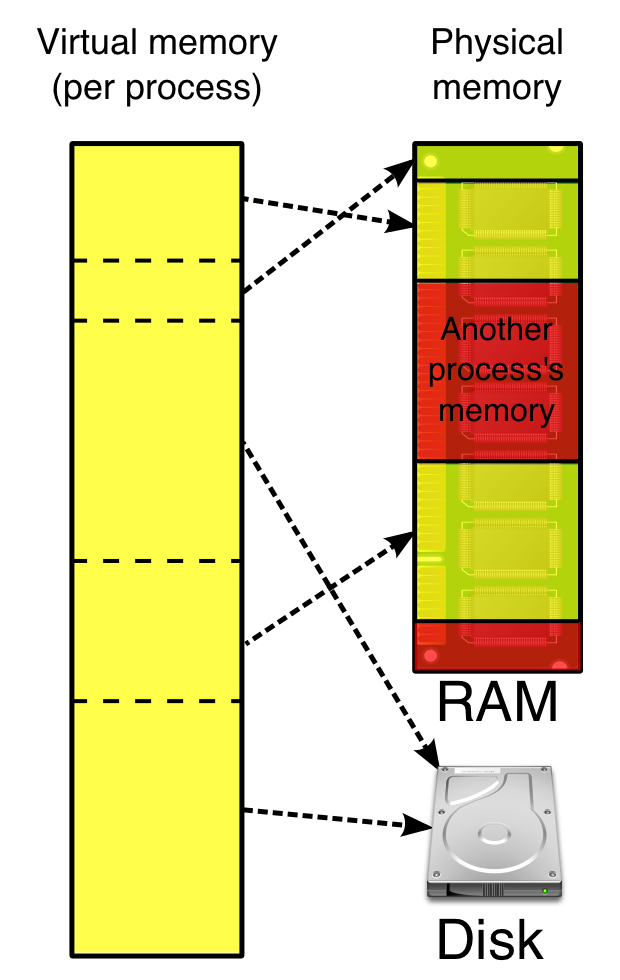
\includegraphics[scale=0.2]{./figures/Virtual_memory.png}
    \end{column}
    \begin{column}{0.7\textwidth}
      \bi
    \item Maps a contiguous virtual address space to physical memory and disk
      \ei
    \end{column}
  \end{columns}
\end{frame}

\begin{frame}{Background: Linux Virtual Memory}
  \begin{center}
    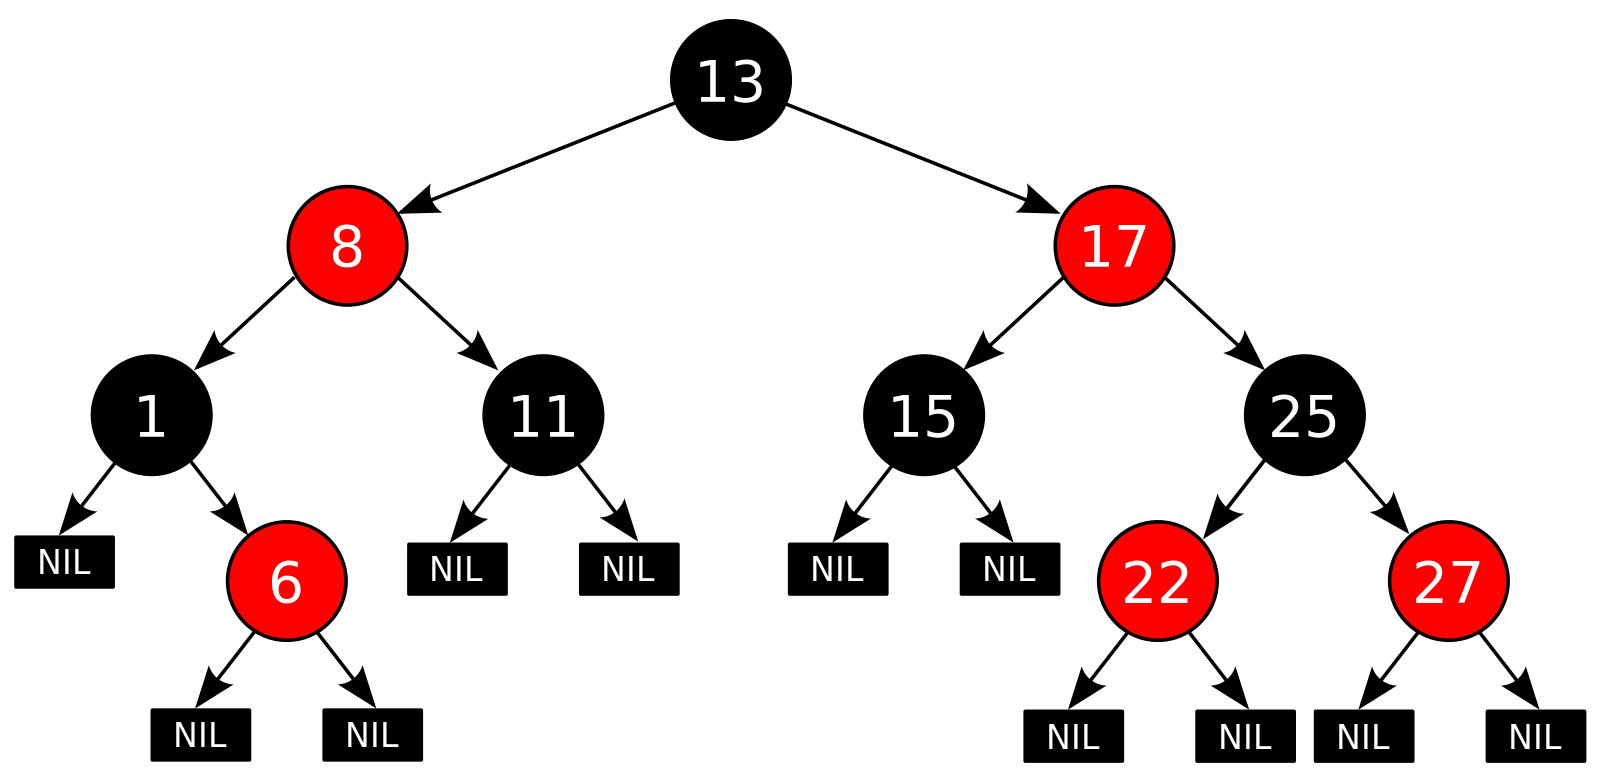
\includegraphics[scale=0.2]{./figures/Red-black_tree.png}
    \bi
    \item Red-black tree
    \item Allows the kernel to search for memory area covering a virtual address
      \pause
    \item \color{red}{Problem: A single lock per address space!}
    \ei
  \end{center}
\end{frame}


% Structuring a talk is a difficult task and the following structure
% may not be suitable. Here are some rules that apply for this
% solution: 

% - Exactly two or three sections (other than the summary).
% - At *most* three subsections per section.
% - Talk about 30s to 2min per frame. So there should be between about
%   15 and 30 frames, all told.

% - A conference audience is likely to know very little of what you
%   are going to talk about. So *simplify*!
% - In a 20min talk, getting the main ideas across is hard
%   enough. Leave out details, even if it means being less precise than
%   you think necessary.
% - If you omit details that are vital to the proof/implementation,
%   just say so once. Everybody will be happy with that.

\begin{frame}[noframenumbering]{References}
\bi
\item Linux VM info from:\\ \url{http://duartes.org/gustavo/blog/post/how-the-kernel-manages-your-memory/}
\ei
\end{frame}

\begin{frame}[noframenumbering]{Attribution}
\bi
\item Virtual memory diagram by Ehamberg (Own work) [CC BY-SA 3.0 (\url{http://creativecommons.org/licenses/by-sa/3.0}) or GFDL (\url{http://www.gnu.org/copyleft/fdl.html})], via Wikimedia Commons
\ei
\end{frame}

\end{document}



